
%(BEGIN_QUESTION)
% Copyright 2014, Tony R. Kuphaldt, released under the Creative Commons Attribution License (v 1.0)
% This means you may do almost anything with this work of mine, so long as you give me proper credit

Calculate the amount of voltage between points A and B in this circuit, and also sketch a phasor diagram showing how all the voltages relate to each other in this circuit:

$$\includegraphics[width=15.5cm]{i00834x01.eps}$$

\underbar{file i00834}
%(END_QUESTION)





%(BEGIN_ANSWER)

First, calculating the voltages between each test point and ground.  $V_A$ is nothing more than the first source's voltage divided by 2 through the resistor network.  $V_B$ is one-third of its source voltage, with an additional 180$^{o}$ phase shift created by the reversed polarity of the secondary winding:

$$V_A = {195 \hbox{ V} \angle 25^o \over 2} = 97.5 \hbox{ V} \angle 25^o$$

$$V_B = {-(220 \hbox{ V} \angle -40^o) \over 3} = 73.33 \hbox{ V} \angle 140^o$$

Sketching both of these quantities on a phasor diagram, we can plot the voltage $V_{AB}$ by the distance between the $V_A$ and $V_B$ phasor lines:

$$\includegraphics[width=15.5cm]{i00834x02.eps}$$

Voltage $V_{AB}$ is simply the difference between $V_A$ and $V_B$:

$$V_{AB} = V_A - V_B$$

$$V_{AB} = (97.5 \hbox{ V} \angle 25^o) - (73.33 \hbox{ V} \angle 140^o)$$

$$V_{AB} = 144.7 \hbox{ V} \angle -2.35^o$$

%(END_ANSWER)





%(BEGIN_NOTES)


%INDEX% Electronics review: AC transformer circuit
%INDEX% Electronics review, phasor expressions of circuit quantities

%(END_NOTES)


